\documentclass[
  bibliography=totoc,     % Literatur im Inhaltsverzeichnis
  captions=tableheading,  % Tabellenüberschriften
  titlepage=firstiscover, % Titelseite ist Deckblatt
]{scrartcl}

% Paket float verbessern
\usepackage{scrhack}

% Warnung, falls nochmal kompiliert werden muss
\usepackage[aux]{rerunfilecheck}

% unverzichtbare Mathe-Befehle
\usepackage{amsmath}
% viele Mathe-Symbole
\usepackage{amssymb}
% Erweiterungen für amsmath
\usepackage{mathtools}

% Fonteinstellungen
\usepackage{fontspec}
% Latin Modern Fonts werden automatisch geladen
% Alternativ:
%\setromanfont{Libertinus Serif}
%\setsansfont{Libertinus Sans}
%\setmonofont{Libertinus Mono}
\recalctypearea % Wenn man andere Schriftarten gesetzt hat,
% sollte man das Seiten-Layout neu berechnen lassen

% deutsche Spracheinstellungen
\usepackage{polyglossia}
\setmainlanguage{german}


\usepackage[
  math-style=ISO,    % ┐
  bold-style=ISO,    % │
  sans-style=italic, % │ ISO-Standard folgen
  nabla=upright,     % │
  partial=upright,   % ┘
  warnings-off={           % ┐
    mathtools-colon,       % │ unnötige Warnungen ausschalten
    mathtools-overbracket, % │
},                       % ┘
]{unicode-math}

% traditionelle Fonts für Mathematik
\setmathfont{Latin Modern Math}
% Alternativ:
%\setmathfont{Libertinus Math}

\setmathfont{XITS Math}[range={scr, bfscr}]
\setmathfont{XITS Math}[range={cal, bfcal}, StylisticSet=1]

% Zahlen und Einheiten
\usepackage[
locale=DE,                   % deutsche Einstellungen
separate-uncertainty=true,   % immer Fehler mit \pm
per-mode=symbol-or-fraction, % / in inline math, fraction in display math
]{siunitx}

% chemische Formeln
\usepackage[
version=4,
math-greek=default, % ┐ mit unicode-math zusammenarbeiten
text-greek=default, % ┘
]{mhchem}

% richtige Anführungszeichen
\usepackage[autostyle]{csquotes}

% schöne Brüche im Text
\usepackage{xfrac}

% Standardplatzierung für Floats einstellen
\usepackage{float}
\floatplacement{figure}{htbp}
\floatplacement{table}{htbp}

% Floats innerhalb einer Section halten
\usepackage[
section, % Floats innerhalb der Section halten
below,   % unterhalb der Section aber auf der selben Seite ist ok
]{placeins}

% Seite drehen für breite Tabellen: landscape Umgebung
\usepackage{pdflscape}

% Captions schöner machen.
\usepackage[
  labelfont=bf,        % Tabelle x: Abbildung y: ist jetzt fett
  font=small,          % Schrift etwas kleiner als Dokument
  width=0.9\textwidth, % maximale Breite einer Caption schmaler
]{caption}
% subfigure, subtable, subref
\usepackage{subcaption}

% Grafiken können eingebunden werden
\usepackage{graphicx}
% größere Variation von Dateinamen möglich
\usepackage{grffile}

% schöne Tabellen
\usepackage{booktabs}

% Verbesserungen am Schriftbild
\usepackage{microtype}

% Literaturverzeichnis
\usepackage[style=alphabetic,]{biblatex}
% Quellendatenbank
\addbibresource{lit.bib}

% Hyperlinks im Dokument
\usepackage[
  unicode,        % Unicode in PDF-Attributen erlauben
  pdfusetitle,    % Titel, Autoren und Datum als PDF-Attribute
  pdfcreator={},  % ┐ PDF-Attribute säubern
  pdfproducer={}, % ┘
]{hyperref}
% erweiterte Bookmarks im PDF
\usepackage{bookmark}

% Trennung von Wörtern mit Strichen
\usepackage[shortcuts]{extdash}

\title{V355: Gekoppelte Schwingkreise}
\author{
  Simon Schulte
  \texorpdfstring{
    \\
    \href{mailto:simon.schulte@udo.edu}{simon.schulte@udo.edu}
  }{}
  \texorpdfstring{\and}{, }
  Tim Sedlaczek
  \texorpdfstring{
    \\
    \href{mailto:tim.sedlaczek@udo.edu}{tim.sedlaczek@udo.edu}
  }{}
}
\publishers{TU Dortmund – Fakultät Physik}

\date{Durchführung: 31.1.2017\\
      Abgabe: 07.02.2017}


\begin{document}

\maketitle
\thispagestyle{empty}
\tableofcontents
\newpage
\section{Theorie}
\label{sec:theorie}
\begin{figure}[htb]
  \centering
  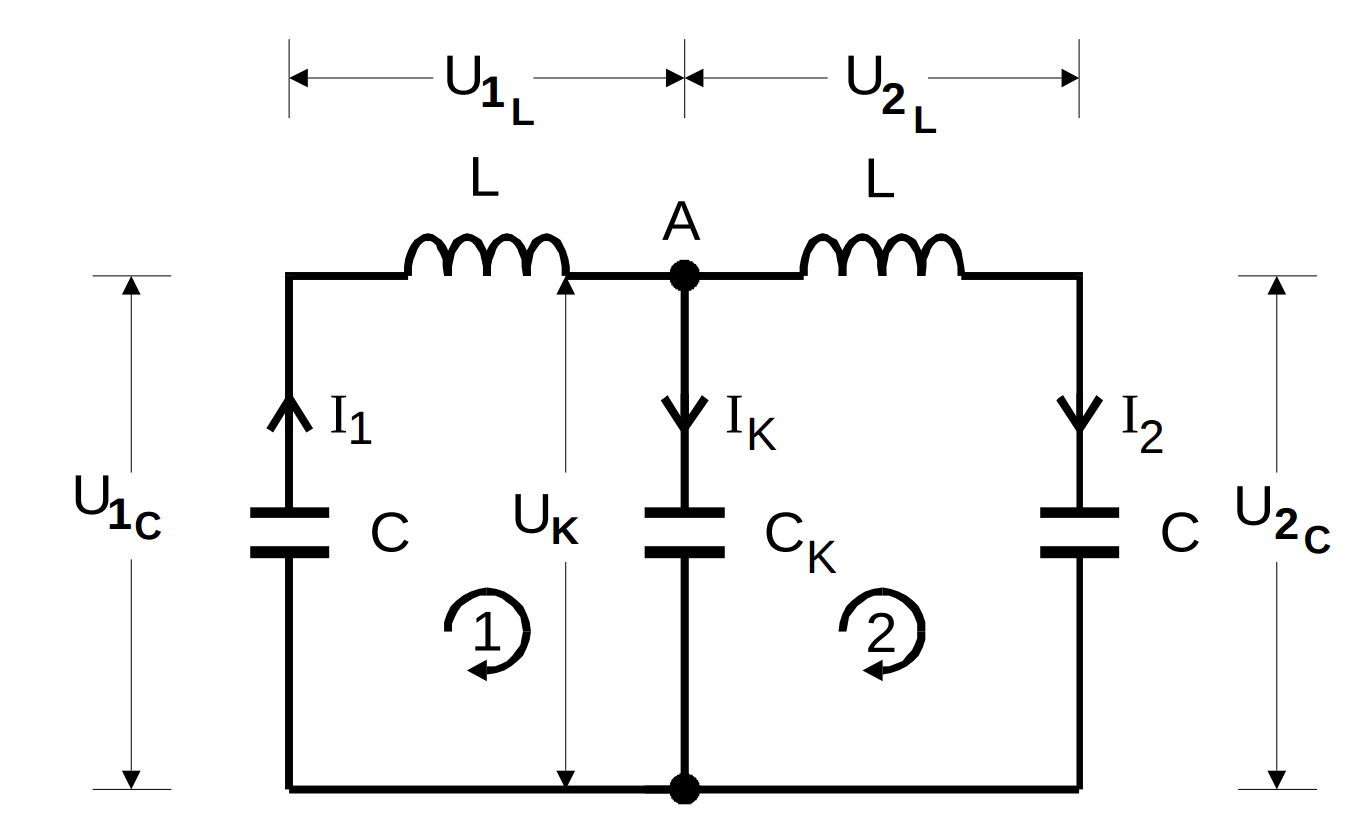
\includegraphics[width=0.85\textwidth]{V3551.png}
  \caption{Der Versuchsaufbau von zwei gekoppelten Schwingkreisen}
  \label{fig:V3551}
\end{figure}
In diesem Versuch werden gekoppelte Schwingkreise im Hinblick auf Energietausch
und auf ihre Fundamentalschwingungen untersucht. In Abbildung 1 zu sehen ist
das Schaltbild zweier kapazitiv gekoppelter Schwingkreise. In diesem Schaltkreis
werden INduktivitäten $L$ und Kapazitäten $C$ verwendet. $C_K$ charakterisiert
dabei den Kopplungskondensator. Mit Hilfe der Kirchhoofschen Regeln lassen
sich dann 2 Schwingungsgleichungen aufstellen. Die Maschenregel ist in der
Abbildung visualisiert für die beiden Maschen 1 und 2. Die beiden
Schwingungsgleichungen lauten:
\begin{align}
  L\frac{\mathup{d}²I_1}{\mathup{d}t²}+\frac{1}{C}I_1+\frac{1}{C_K}(I_1-I_2)=0 \\
  L\frac{\mathup{d}²I_2}{\mathup{d}t²}+\frac{1}{C}I_2-\frac{1}{C_K}(I_1-I_2)=0.
  \label{eqn:schwingungsgleichungen}
\end{align}
Wenn man Gleichung (1) und Gleichung (2) subtrahiert folgt:
\begin{align}
  L\frac{\mathup{d}²}{\mathup{d}t²}(I_1+I_2)+\frac{1}{C}(I_1+I_2)=0 \\
  L\frac{\mathup{d}²}{\mathup{d}t²}(I_1-I_2)+(\frac{1}{C}+\frac{2}{C_K})(I_1-I_2)=0.
\end{align}
Die Subtraktion wird durchgeführt, damit die beiden Differentialgleichungen nicht
mehr voneinander abhängig sind. Nun ist es möglich beide unabhängig voneinander
zu lösen. Als Lösung für Gleichung 3 folgt eine harmonische Schwingung, welche
als gleichphasig bezeichnet wird. Beide Schwingkreise schwingen dabei so, als
wäre keine Kopplung vorhanden. Es verhält sich dann als zwei Schwingkreise, die
mit gleicher Amplitude und Phase anfangen zu oszillieren. Die
Schwingungsfrequenz dieser ist definiert durch:
\begin{equation}
  \nu_+=\frac{1}{2\pi\sqrt{LC}}.
\end{equation}
Bei einer gegenphasigen Schwingung beginnt die Oszillation mit gleicher
Amplitude und einer entgegengesetzten Phase. Die Schwingungsfrequenz dieser
ist definiert durch:
\begin{equation}
  \nu_-=\frac{1}{2\pi\sqrt{L(\frac{1}{C}+\frac{2}{C_K})^{-1}}}.
\end{equation}
$\nu_+$ und $\nu_-$ sind die Frequenzen zu den Fundamentalschwingungen des
gekoppelten Systems, wobei die folgende Ungleichung gilt:
\begin{equation}
  \nu_->\nu_+
\end{equation} \\
\\
Die erste Masche aus Abbildung \ref{fig:V3551} hat zum Zeitpunkt $t=0$ einen
Strom von ungleich 0. Dann hat die Amplitude der ersten Schwingung genau dann
ein Maximum, wenn die Amplitude der zweiten Schwingung gleich 0 ist. Es
ergibt sich dann aus den Gleichungen 3 und 4:
\begin{align}
  I_1(t) &=I_{1_0}\cos(\frac{1}{2}(\omega_++\omega_-)t)\cos(\frac{1}{2}(\omega_+-\omega_-)t) \\
  I_2(t) &=I_{1_0}\sin(\frac{1}{2}(\omega_++\omega_-)t)\sin(\frac{1}{2}(\omega_+-\omega_-)t).
\end{align}
Im Verlauf der Zeit wird $I_2$ größer und $I_1$ kleiner, bis zu dem Zeitpunkt, andem
die Ausgangslage umgekehrt wurde. Außerdem wird die Annahme getroffen, dass
$C_K>>C$ gilt und damit auch:
\begin{align}
  \frac{1}{2}(\omega_++\omega_-)\thickapprox\omega_+ \\
  \omega_-\omega_+<<\omega_+.
\end{align}
\begin{figure}[htb]
  \centering
  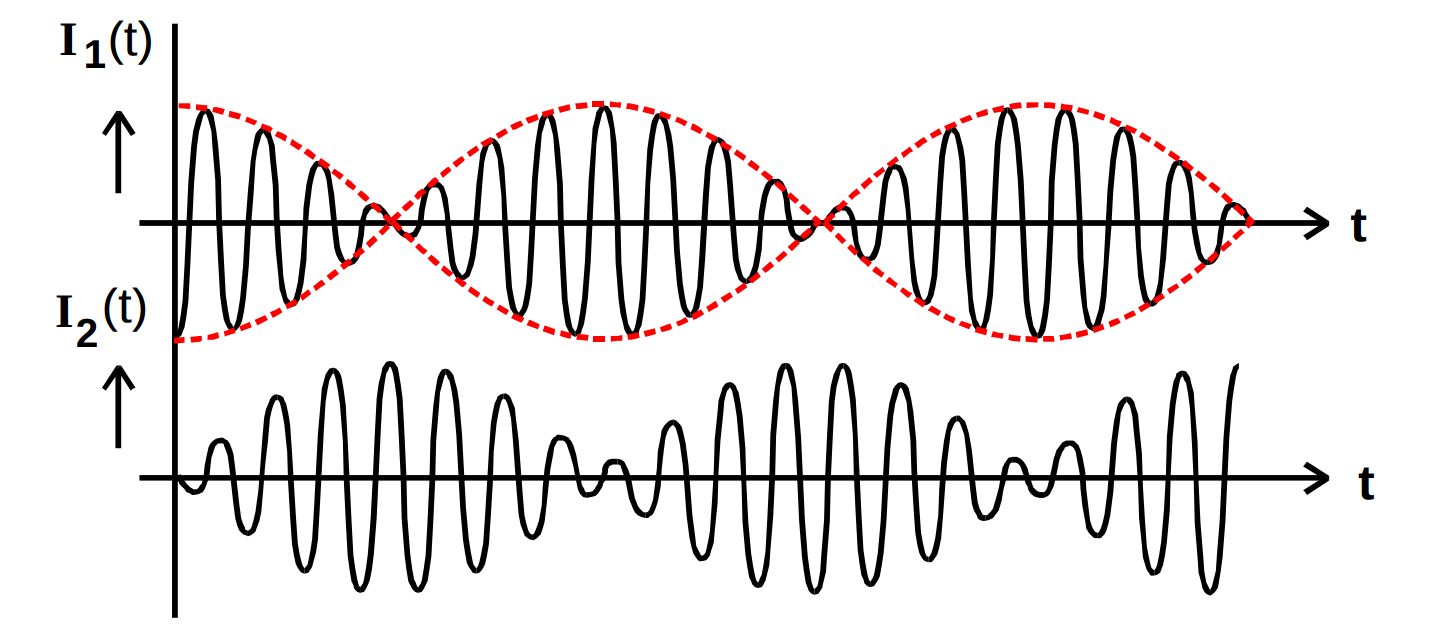
\includegraphics[width=0.85\textwidth]{V3552.png}
  \caption{Der Amplitudenverlauf von zwei Schwingungen überlagert mit einer Schwebung}
  \label{fig:V3552}
\end{figure}
In Abbildung \ref{fig:V3552} zu sehen ist dann der Amplitudenverlauf zweier
Schwingungen, wenn eine Schwebung eintritt, wie durch die vorherigen Gleichungen
beschrieben. Dabei wird die Frequenz $\nu_--\nu_+$ als Schwebungsfrequenz
bezeichnet. Die Schwebungsfrequenz ist die Frequenz, mit der die Gesamtenergie
des Systems zwischen den Schwingkreisen oszilliert.
\section{Durchführung}
\label{sec:durchführung}

\subsection{Versuchsaufbau}
\label{sec:versuchsaufbau}
\begin{figure}[htb]
  \centering
  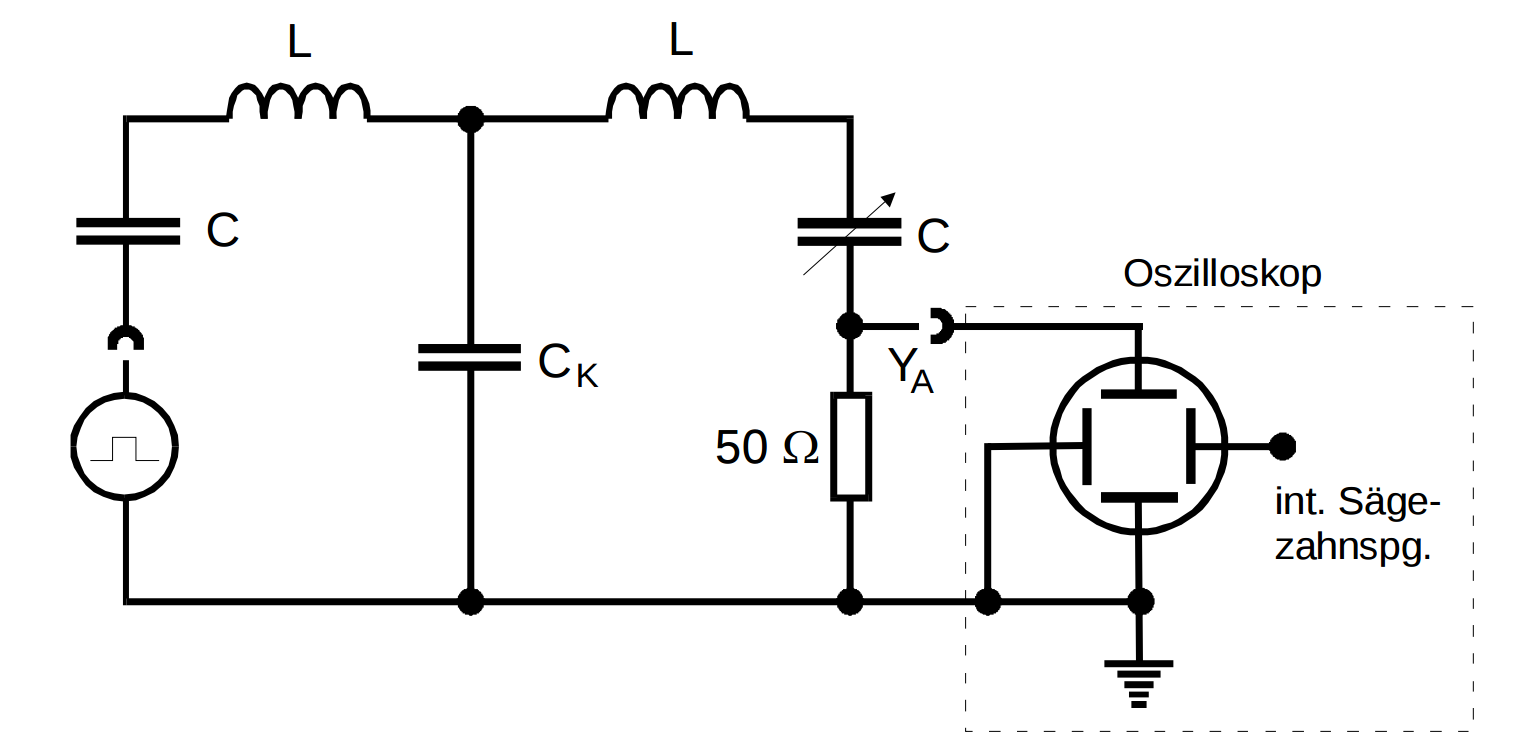
\includegraphics[width=0.85\textwidth]{V3554.png}
  \caption{Der zur Untersuchung des Schwebungsphänomens und der Fundamentalschwingungen verwendete Versuchsaufbau. Für die Messung der Fundamentalschwingungen wurden kleine Änderungen an dem Schaltkreis vorgenommen.}
  \label{fig:V3554}
\end{figure}
In Abbildung \ref{fig:V3554} zu sehen ist der genutzte Versuchsaufbau zur
Untersuchung des Schwebungsphänomens und, mit leichten Abwandlungen, zur
Ermittlung der Fundamentalschwingungen. Dabei wird mit einer Rechteckspannung
Masche 1 angeregt. Über den Kopplungskondensator $C_K$ gelangt dann
die Schwingung in die zweite Masche des gekoppelten Schwingkreises. Dort wird
über den Ohmschen Widerstand beim Oszilloskop die Schwebung sich2tbar gemacht.
Danach werden die Fundamentalschwingungen bestimmt. Dazu wird die Rechteckspannung
mit einer Sinusspannung ersetzt.
\subsection{Versuchsdurchführung}
\label{sec:versuchsdurchführung}
\begin{figure}[htb]
  \centering
  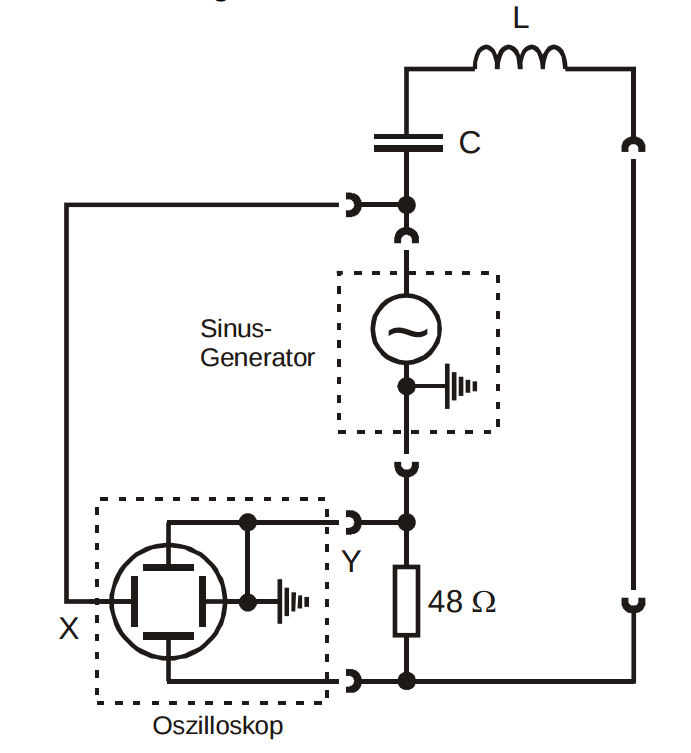
\includegraphics[width=0.75\textwidth]{V3553.png}
  \caption{Versuchsaufbau zur Justierung des einstellbaren Kondensators}
  \label{fig:V3553}
\end{figure}
In Abbildung \ref{fig:V3553} zu sehen ist die Schaltskizze zur Justierung
des einstellbaren Kondensators von Masche 2 aus Abbildung \ref{fig:V3554}
Justiert wird dabei der Schwingkreis aus Abbildung \ref{fig:V3554} auf die
Resonanzfrequenz des anderen Schwignkreises. Dafür sucht man mit Hilfe von
Lissajous-Figuren, die auf dem Oszilloskop zu sehen sind, die Frequenz, bei der
die Phase zwischen Generatorspannung und Schwingkreisstrom in Masche 1
gleich $\frac{\pi}{2}$ ist. Danach wird der Vorgang für Masche 2 wiederholt, mit
dem Unterschied, dass nun die zuvor bestimmte Resonanzfrequenz durch den
verstellbaren Kondensator eingestellt wird. \\
\\
Nach der Justierung wird dann als erstes das Verhältnis zwischen Schwingungsfrequenz
und Schwebungsfrequenz bestimmt. Dafür wird die Anzahl der Schwingungsmaxima
innerhalb einer Schwebungsperiode für $2\,\leq\,C_K\,\leq\,12\,nF$, für den
Kopplungskondensator, gemessen. \\
\\
Danach werden die beiden Fundamentalschwingungen $\nu_-$ und $\nu_+$ bestimmt.
Auch hier wird die Kapazität des Kopplungskondensators zwischen
$2\,\leq\,C_K\,\leq\,12\,nF$ variiert. Es werden zur Messung Sinusspannung
und Schwingkreisstrom im Oszilloskop gegeneinander aufgetragen. Dann wird
mit Hilfe von Lissajous-Figuren genau die Frequenz gesucht, ber der die
jeweilige Phase 0, für $\nu_+$, oder $\pi$, für $\nu_-$ wird.\\
\\
Als letztes werden erneut, abhängig von $2\,\leq\,C_K\,\leq\,12\,nF$, die beiden
Fundamentalschwingungen bestimmt. Dafür wird allerdings jetzt der Sweep genutzt.
Beim Sweep wird in einer Sekunde das Frequenzsprektrum einer beliebigen
Anfangsfrequenz bis zu einer, ebenfalls beliebigen, Endfrequenz auf dem
Oszilloskop sichtbar gemacht. Primär sichtbar sind dann zwei große Peaks,
die die Frequenzen $\nu_+$ und $\nu_-$ darstellen.\\
\\
Es wurde Schaltung 2 genutzt mit den folgenden Bauteilwerten:
\begin{align}
  L=\SI{23.954}{mF} \\
  C=\SI{0.7932}{nF} \\
  C_{sp}=\SI{0.028}{nF}
\end{align}
Dabei gibt $C_sp$ die Spuleneigene Kapazität an.
\end{document}
